\documentclass[12pt]{book}

\usepackage{amsmath, amssymb, amsthm}
\usepackage{graphicx}
\usepackage{hyperref}
\usepackage{fancyhdr}
\usepackage{titlesec}
\usepackage{geometry}
\usepackage{setspace}
\usepackage{xcolor}
\usepackage{newunicodechar}
\newunicodechar{✓}{\checkmark}
\setlength{\headheight}{15pt} % silences fancyhdr warning
\usepackage{tikz}
\usepackage{listings}
\usepackage{float} % For [H] figures


\lstset{
  basicstyle=\ttfamily\small,
  breaklines=true,
  breakatwhitespace=true,
  columns=fullflexible,
  inputencoding=utf8,
  extendedchars=true,
  literate={✓}{{\checkmark}}1 {✅}{{\checkmark}}1
}


\geometry{margin=1in}
\onehalfspacing

% Fancy headers
\pagestyle{fancy}
\setlength{\headheight}{15pt}
\addtolength{\topmargin}{-2pt}
\fancyhf{}
\fancyhead[L]{COMSC 2043: Induction and Recursion}
\fancyhead[R]{\thepage}

% Chapter style
\titleformat{\chapter}[display]
  {\normalfont\bfseries\Huge\color{blue!60!black}}
  {\chaptername\ \thechapter}{20pt}{\Huge}

\title{
  \vspace{2cm}
  \textbf{COMSC 2043}\\
  \textbf{Induction and Recursion}\\[1em]
  \Large Student Workbook
  \vspace{1cm}
}

\author{Jeremy Evert \\ Southwestern Oklahoma State University}
\date{\today}

\begin{document}
\maketitle
\tableofcontents
\clearpage

\chapter{Foundations of Induction and Recursion}

This chapter introduces the central ideas of \textbf{mathematical induction} and \textbf{recursion} as presented in Chapter 5 of Kenneth Rosen's \emph{Discrete Mathematics and Its Applications}.

\section{The Big Picture}

Mathematical induction and recursion are two sides of the same elegant coin. Induction is how we \emph{prove} things about a process that repeats. Recursion is how we \emph{define} that process.

We use induction to reason that what works for one step will work for the next. We use recursion to build structures or compute results by defining a problem in terms of smaller instances of itself.

\section{Key Ideas from Rosen’s Chapter 5}

\begin{itemize}
  \item \textbf{Basis Step:} Prove that a statement is true for an initial value (usually $n=0$ or $n=1$).
  \item \textbf{Inductive Step:} Assume it is true for $n=k$ (the \emph{inductive hypothesis}) and prove it for $n=k+1$.
  \item \textbf{Strong Induction:} Sometimes we assume it’s true for \emph{all} previous cases up to $k$ to prove it for $k+1$.
  \item \textbf{Recursive Definitions:} A way to define sets, sequences, or functions in terms of themselves.
  \item \textbf{Structural Induction:} A generalization used for recursively defined structures like trees or expressions.
\end{itemize}

\section{Why This Matters}

Induction teaches us to trust the domino effect: if one falls and the rule is consistent, they all fall. Recursion lets us \emph{build the dominoes} themselves.

They are the grammar and logic behind everything from factorial functions to sorting algorithms to proofs of algorithmic correctness.

\section{Example: The Factorial Function}

The factorial of $n$, written $n!$, is defined recursively:
\[
  n! = 
  \begin{cases}
    1, & n = 0 \\
    n \cdot (n-1)!, & n > 0
  \end{cases}
\]

We can prove by induction that $n! \ge 2^{n-1}$ for all $n \ge 1$.

\textbf{Proof (sketch):}
\begin{itemize}
  \item \textbf{Base case:} When $n = 1$, we have $1! = 1 \ge 2^{0} = 1$\,\checkmark
  \item \textbf{Inductive step:} Assume $k! \ge 2^{k-1}$ for some integer $k \ge 1$. Then
  \[
      (k+1)! = (k+1)\,k! \ge (k+1)2^{k-1} \ge 2^{k}.
  \]
  Therefore, the inequality holds for $k + 1$, completing the induction.
\end{itemize}

\section{A Student Challenge}

\begin{quote}
“Induction is not a leap of faith — it’s a method of climbing an infinite ladder, one rung at a time.”
\end{quote}

\textbf{Challenge:} Write your own recursive function in Python that computes $n!$, and then write a proof by induction showing why it works for all $n \ge 0$.

\section{Checkpoint Questions}
\begin{enumerate}
  \item What are the two main steps of a proof by induction?
  \item How is recursion related to induction?
  \item Give a real-world example of a recursive process.
  \item Can every recursive definition be proven correct using induction?
\end{enumerate}


\chapter{Recursive Algorithms}

Recursion is the heartbeat of algorithmic thinking.  
It allows us to describe a complex process in terms of smaller, self-similar pieces.  
In this chapter, we’ll explore how to turn recursive definitions into recursive algorithms.

\section{From Definition to Algorithm}

A recursive algorithm solves a problem by reducing it to smaller instances of the same problem.
Every recursive algorithm must include:

\begin{enumerate}
  \item \textbf{Base Case:} a simple situation that can be solved directly.
  \item \textbf{Recursive Case:} a rule for breaking the problem into smaller subproblems.
  \item \textbf{Convergence:} assurance that each recursive call moves toward the base case.
\end{enumerate}

\section{Example: Summation}

Let us define a function that computes the sum of the first $n$ natural numbers:

\[
S(n) =
\begin{cases}
0, & n = 0 \\
n + S(n-1), & n > 0
\end{cases}
\]

\noindent
\textbf{Recursive Algorithm (Python style):}

\begin{verbatim}
def sum_to_n(n):
    if n == 0:
        return 0
    else:
        return n + sum_to_n(n - 1)
\end{verbatim}

Each recursive call reduces $n$ by one until it reaches the base case $n = 0$.
This process mirrors the inductive definition of summation.

\section{Example: Factorial Function}

We can express $n!$ recursively as:
\[
n! =
\begin{cases}
1, & n = 0,\\
n \cdot (n-1)!, & n > 0.
\end{cases}
\]

\noindent
\textbf{Recursive Algorithm:}
\begin{verbatim}
def factorial(n):
    if n == 0:
        return 1
    else:
        return n * factorial(n - 1)
\end{verbatim}

Each call creates a new stack frame that holds the current value of $n$ until the base case is reached.
When the recursion unwinds, the frames multiply their stored $n$ values in reverse order.

\section{Example: Fibonacci Sequence}

The Fibonacci sequence is defined by
\[
F(n) =
\begin{cases}
0, & n = 0,\\
1, & n = 1,\\
F(n-1) + F(n-2), & n > 1.
\end{cases}
\]

\noindent
\textbf{Recursive Algorithm:}
\begin{verbatim}
def fib(n):
    if n <= 1:
        return n
    else:
        return fib(n - 1) + fib(n - 2)
\end{verbatim}

This version is beautifully simple but computationally explosive—each call spawns two more.
For large $n$, this algorithm grows exponentially in time.
We will later optimize it using \textbf{memoization} and \textbf{iteration}.

\section{Tracing a Recursive Call}

Let us trace the computation of \texttt{sum\_to\_n(4)}:

\[
S(4) = 4 + S(3) = 4 + (3 + S(2)) = 4 + 3 + 2 + 1 + S(0) = 10
\]

\noindent
During recursion, a \emph{call stack} forms:
\[
S(4) \rightarrow S(3) \rightarrow S(2) \rightarrow S(1) \rightarrow S(0)
\]
and then unwinds back in the reverse order as results return upward.

\section{Analyzing Recursive Cost}

The cost of recursion depends on the number of calls and the work per call.
For the factorial function, the recurrence relation is:
\[
T(n) = T(n-1) + O(1),
\]
which resolves to $O(n)$.
For Fibonacci, the recurrence
\[
T(n) = T(n-1) + T(n-2) + O(1)
\]
yields $O(2^n)$ — a dramatic difference.

\section{Challenge Problems}

\begin{enumerate}
  \item Write a recursive algorithm for computing the sum of digits of an integer.
  \item Modify the Fibonacci algorithm to use memoization.  
  \item Trace the recursion tree of \texttt{fib(5)} and count the total number of calls.
  \item Prove by induction that your optimized Fibonacci algorithm runs in $O(n)$ time.
\end{enumerate}

\begin{quote}
``A recursive algorithm is not just a loop—it is a story told backward and forward at the same time.''
\end{quote}


\chapter{The Fibonacci Sequence — Nature’s Algorithm}

\section{The Story of Fibonacci}
Long ago, in a quiet Italian village, a mathematician named Leonardo of Pisa—nicknamed \textbf{Fibonacci}—noticed patterns in nature that seemed to whisper numbers into every petal, every pinecone, every spiral galaxy.

The Fibonacci sequence begins simply:
\[
F(0) = 0, \quad F(1) = 1,
\]
and each term afterwards is born from the sum of its two predecessors:
\[
F(n) = F(n-1) + F(n-2).
\]
So, the sequence grows:
\[
0, \; 1, \; 1, \; 2, \; 3, \; 5, \; 8, \; 13, \; 21, \; 34, \ldots
\]

Each generation in this sequence depends upon the previous two—just as branches split from branches, and ideas sprout from ideas.

\vspace{1em}
\begin{center}
\textit{Recursion is nature’s favorite loop.}
\end{center}
\vspace{1em}

\section{Seeing the Pattern}
To visualize how recursion unfolds, consider the computation of $F(5)$:

\[
\texttt{fib(5)} \rightarrow \texttt{fib(4)} + \texttt{fib(3)}
\]

Each call branches into two smaller ones, creating a beautiful tree of self-reference:

\begin{center}
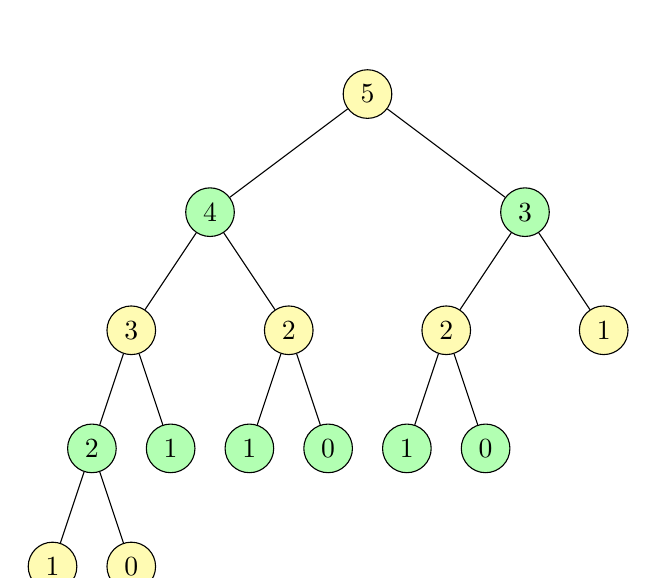
\begin{tikzpicture}[level distance=1.5cm,
  level 1/.style={sibling distance=4cm},
  level 2/.style={sibling distance=2cm},
  level 3/.style={sibling distance=1cm}]
  \node[circle,draw,fill=yellow!30]{5}
    child {node[circle,draw,fill=green!30]{4}
      child {node[circle,draw,fill=yellow!30]{3}
        child {node[circle,draw,fill=green!30]{2}
          child {node[circle,draw,fill=yellow!30]{1}}
          child {node[circle,draw,fill=yellow!30]{0}}}
        child {node[circle,draw,fill=green!30]{1}}}
      child {node[circle,draw,fill=yellow!30]{2}
        child {node[circle,draw,fill=green!30]{1}}
        child {node[circle,draw,fill=green!30]{0}}}}
    child {node[circle,draw,fill=green!30]{3}
      child {node[circle,draw,fill=yellow!30]{2}
        child {node[circle,draw,fill=green!30]{1}}
        child {node[circle,draw,fill=green!30]{0}}}
      child {node[circle,draw,fill=yellow!30]{1}}};
\end{tikzpicture}
\end{center}

Notice how each recursive call duplicates work from previous branches.  
This inefficiency is the price of elegance—but later, we’ll learn to make it faster.

\section{A Gentle Python Introduction}

\begin{verbatim}
def fib_recursive(n):
    """Return the nth Fibonacci number using recursion."""
    if n <= 1:
        return n
    return fib_recursive(n - 1) + fib_recursive(n - 2)

for i in range(10):
    print(f"F({i}) = {fib_recursive(i)}")
\end{verbatim}

Let’s unpack what happens.  
When you call \texttt{fib\_recursive(5)}, the function calls itself twice,  
then each of those calls calls itself twice more,  
until it reaches the \textbf{base cases} where $n = 0$ or $n = 1$.

Each branch blooms, divides, and resolves—just like the petals of a sunflower spiraling toward the sun.

\section{Recursive Beauty}
Recursion is powerful because it mirrors the way we define patterns in nature:  
each step depends upon smaller, simpler versions of itself.

\begin{quote}
\textit{To understand recursion, one must first understand recursion.}
\end{quote}

This idea is both a mathematical truth and a philosophical koan.  
In the next chapters, we’ll measure just how costly this beauty is,  
and how algorithmic growth behaves as $n$ increases.

\begin{center}
\textbf{Coming soon:}\\
\textit{Chapter 4 — Measuring the Cost of Recursion}\\
\textit{and}\\
\textit{Chapter 5 — Understanding Big-O Through Fibonacci.}
\end{center}


\chapter{Measuring the Cost of Recursion}

\section{Purpose}
In this chapter, we investigate how recursive and iterative algorithms differ in their computational cost. Using the Fibonacci sequence as our case study, we’ll see how recursion can sometimes explode in complexity.

\section{The Experiment}
We designed a Python experiment that measures:
\begin{itemize}
  \item The number of function calls
  \item The number of additions
  \item The number of variable assignments
  \item The time required to compute $F_n$
\end{itemize}

\subsection{The Tracker Class}
\lstinputlisting[language=Python, caption={DataTracker and Fibonacci comparison}, label={lst:fib_analysis}]{chapters/fib_analysis.py}

\subsection{Generated Data}
After running the Python code, the script produces two files:
\begin{itemize}
  \item \texttt{fib\_results.csv} — tabular data of timing and operation counts
  \item \texttt{fib\_results\_plot.pdf} — visualization of recursive vs iterative performance
\end{itemize}

\section{Results}
\begin{figure}[H]
    \centering
    \includegraphics[width=\textwidth]{chapters/fib_results_plot.pdf}
    \caption{Recursive vs. Iterative Fibonacci performance}
\end{figure}

\section{Reflection}
Discuss:
\begin{itemize}
  \item Why does the recursive version slow down so dramatically?
  \item How might memoization or dynamic programming fix this?
  \item What do you notice about the patterns of function calls?
\end{itemize}

\section{Student Task}
Run the experiment on your own system. 
Then modify \texttt{fib\_recursive} to include memoization and compare your results.


\chapter{Code Appendix – Fibonacci Source Files}

\section{Overview}
This appendix provides a complete snapshot of the Python source code used in this workbook. 
Each time you rebuild the book, the latest version of the code is automatically included — 
ensuring this text remains a living record of our experiments.

\section{Fibonacci Analysis Script}

\lstset{
  language=Python,
  basicstyle=\ttfamily\footnotesize,
  keywordstyle=\color{blue},
  stringstyle=\color{orange},
  commentstyle=\color{gray},
  numbers=left,
  numberstyle=\tiny\color{gray},
  stepnumber=1,
  frame=single,
  breaklines=true,
  showstringspaces=false,
  tabsize=4,
  captionpos=b
}

\lstinputlisting[
  caption={\texttt{fib\_analysis.py} — A fully instrumented Fibonacci analysis with timing and operation counts.},
  label={lst:fib_analysis_full}
]{chapters/fib_analysis.py}


\chapter{Understanding Big-O Through Fibonacci}
\label{ch:big-o-fib}

\section{Why Fibonacci is the Perfect Big-O Lens}
Fibonacci exposes two very different growth stories:
\begin{itemize}
  \item The naive recursive version has \emph{exponential} time, roughly $O(2^n)$.
  \item With memoization (or bottom-up DP), the time drops to \emph{linear}, $O(n)$, with $O(n)$ space.
\end{itemize}
This makes it a great stage to see how algorithm design transforms cost. \,\,\textit{(See Chapters 2--4 for setup and experiments.)} :contentReference[oaicite:0]{index=0}

\section{Deriving the Cost}
\subsection{Naive recursion: $O(2^n)$ time}
Define the cost $T(n)$ of
\[
F(n)=
\begin{cases}
0,& n=0\\
1,& n=1\\
F(n-1)+F(n-2),& n>1
\end{cases}
\]
Each call to $F(n)$ triggers two subcalls (except at base cases). A standard bound is
\[
T(n)=T(n-1)+T(n-2)+O(1) \quad \Rightarrow \quad T(n)=\Theta(\varphi^n),
\]
where $\varphi=\frac{1+\sqrt{5}}{2}\approx1.618$ and $\varphi^n=\Theta(2^n)$.
Intuition: the recursion tree doubles “enough” times that the total work explodes exponentially.

\subsection{Memoization: $O(n)$ time, $O(n)$ space}
Top-down memoization stores previously computed $F(k)$ so each $k\in\{0,\dots,n\}$ is computed once:
\[
T(n)=T(n-1)+O(1), \quad \text{amortized over } n \text{ distinct subproblems} \Rightarrow T(n)=O(n).
\]
Space is $O(n)$ for the table/stack (top-down) or just $O(n)$ array (bottom-up). The iterative two-variable version achieves $O(1)$ extra space.

\section{Visual: Exponential vs Linear}
Figure~\ref{fig:bigocurves} plots $2^n$ against $n$. The lines start friendly, then $2^n$ rockets away like a bottle rocket with a PhD.
\begin{figure}[htbp]
  \centering
  \includegraphics[width=.85\textwidth]{chapters/big_o_curves.pdf}
  \caption{$2^n$ vs $n$ on the same axes (log-scale optional).}
  \label{fig:bigocurves}
\end{figure}

\section{Code: Three Flavors of Fibonacci}
We include three implementations and an experiment harness that writes CSV and plots.

\subsection{Tracker and Implementations}
\lstinputlisting[language=Python,caption={Tracker and Fibonacci variants},label={lst:fib_variants}]{chapters/fib_variants.py}

\subsection{Experiment: timing, counts, and plots}
\lstinputlisting[language=Python,caption={Benchmark and plots for recursive vs memo vs iterative},label={lst:fib_bench}]{chapters/fib_bench.py}

\section{Practical Implications}
\begin{itemize}
  \item \textbf{Naive recursion} demonstrates explosive growth; great teaching tool, terrible production tool beyond modest $n$.
  \item \textbf{Memoization} replaces recomputation with table lookups: a tiny idea with huge consequences.
  \item \textbf{Iterative DP} keeps the wins while minimizing memory; for Fibonacci, two scalars suffice.
\end{itemize}

\section{Optional: Memory Probe (Laptop)}
To show that Big-O is a map (not the terrain), we sample real memory/CPU while the naive version gnaws on the stack. See Listing~\ref{lst:fib_memprobe}.
\lstinputlisting[language=Python,caption={Lightweight memory/CPU probe while running recursion},label={lst:fib_memprobe}]{chapters/fib_memprobe.py}

\section{Student Prompts}
\begin{enumerate}
  \item For which $n$ does naive recursion become impractical on your machine?
  \item Modify memoization to bottom-up; compare peak memory with \texttt{tracemalloc}.
  \item Explain why memoization changes the recursion tree’s shape and total nodes visited.
\end{enumerate}




% \input{chapters/ch03_fibonacci.tex}
% \input{chapters/ch04_examples.tex}
% \input{chapters/ch05_merge_sort.tex}

\end{document}

